\chapter{Architettura di un Elaboratore}

Questo non è il primo capitolo che viene trattato nel corso, tuttavia per mantenere un ordine migliore è importante comprendere il funzionamento dell'hardware in quanto il sistema operativo ci interagisce strettamente.

Parte degli argomenti del capitolo sono già stati studiati durante il corso di Architettura degli Elaboratori vengono poi introdotti i sistemi multiprocessori, la cui gestione occuperà parte significativa del corso.

\section{Central Processing Unit}

Il compito della CPU è quello di \textbf{eseguire i programmi} immagazzinati nella memoria centrale, leggendo le loro istruzioni ed eseguendole in sequenza.

La CPU opera in modo ciclico, ripetendo fino alla fine del programma le operazioni di \textbf{fetch-decode-execute}: acquisisce l'istruzione, la decodifica e la esegue

\begin{figure}[H]
    \centering
    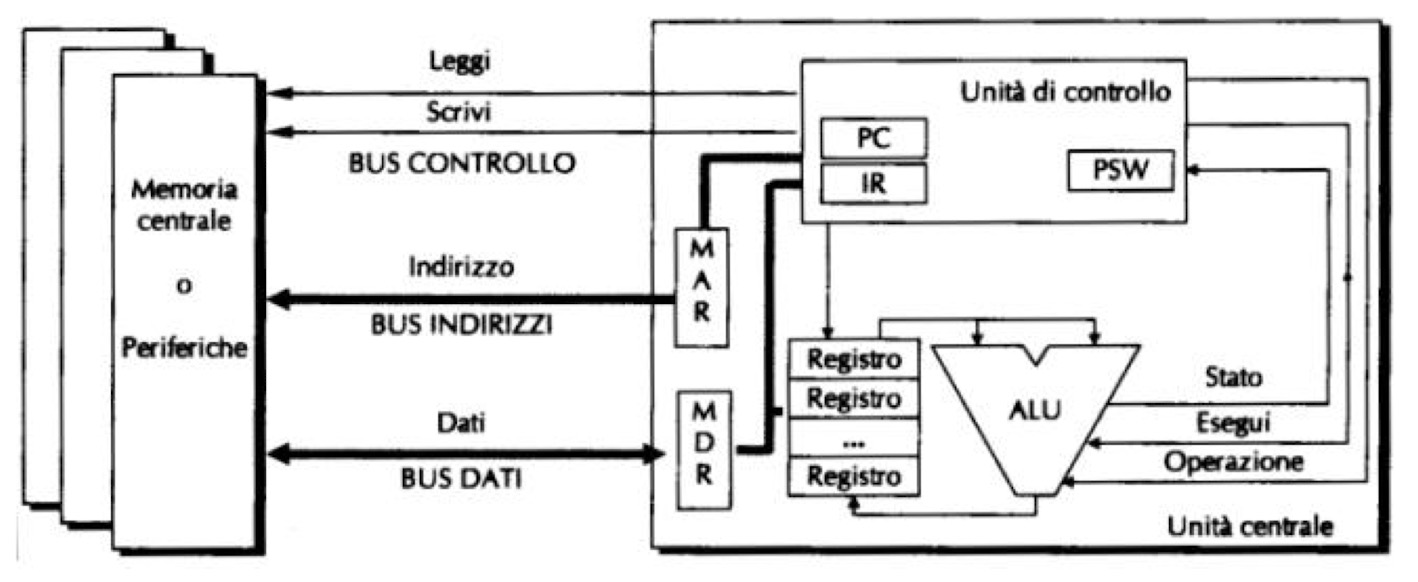
\includegraphics[width=0.55\linewidth]{assets/cpu-architecture.jpg}
\end{figure}

Una CPU è composta da:
\begin{sitemize}
    \item \textbf{Unità di controllo:} ha il compito di leggere le istruzioni e determinarne il tipo.
    \item \textbf{Arithmentic and Logic Unit (ALU):} Esegue le operazoni matematiche necessarie per l'esecuzione dell'istruzione.

    I dati devono partire dai registri e il risultato deve tornare nei registri, questo percorso viene detto \textit{data path}, ogni istruzione comporta l'esecuzione di uno o più cicli di \textit{data path}.
    \item \textbf{Registri:} Una memoria di piccole dimensioni che risiede all'interno del processore, viene utilizzata per memorizzare i risultati temporanei e le informazioni di controllo della CPU.

    \begin{note}
        Due registri particolarmente importanti sono l'Instruction Register (IR) che immagazzina l'istruzione corrente e il Program Counter (PC) che punta alla prossima istruzione.
    \end{note}

    \item \textbf{MDR:} è un registro a cui la ALU ha accesso diretto e che contiene momentaneamente i dati da/per la CPU.
    \item \textbf{MAR:} è un registro della CPU contenente l'indirizzo della locazione di memoria RAM in cui si andrà a leggere o scrivere un dato.
    \item \textbf{Bus di Controllo:} un bus che permette alla CPU di specificare che operazione deve svolgere sulla memoria.
    \item \textbf{PSW:} \textit{Program Status Word} i bit che forniscono informazioni sul risultato dell'ultima operazione eseguita. (overflow, carry, segno)
\end{sitemize}

Ogni ciclo di esecuzione si compone di alcuni passaggi:
\begin{sitemize}
    \item Il valore di PC viene copiato nel MAR
    \item La memoria scrive sul MDR il valore all'indice specificato dal MAR
    \item Il valore di MDR viene copiato sull'IR
    \item L'istruzione viene eseguita dall'ALU
    \begin{sitemize}
        \item Se l'istruzione richiede degli operandi essi devono essere inseriti nei registri attraverso MAR e MDR, similmente a quanto fatto per l'istruzione
    \end{sitemize}
    \item Terminata l'esecuzione il risultato viene scritto sul MDR e l'indirizzo di destinazione sul MAR, la memoria poi si occupa di copiare il valore.
    \item Si ricomincia dal primo punto con l'istruzione successiva.
\end{sitemize}

\section{Prestazioni di un Elaboratore}

Sia un processore con una frequenza di clock $F$ e quindi con periodo di clock $T = \frac{1}{F}$. Questo è il tempo necessario per eseguire un ciclo di \textit{data path}.

\subsubsection*{Istruzioni al secondo}
Per svolgere un'istruzione che richiede $n$ cicli di \textit{data path} $t_{i} = n \cdot T$

Quindi il numero di istruzioni processate al secondo sarà $N = \frac{1}{t_{i}} = \frac{F}{n}$

\subsubsection*{Tempo di esecuzione di un processo}
$$T_{es} = T \cdot (\sum_{i=1}^n N_i \cdot CPI_i )$$

Dove $N_i$ è il numero di istruzioni di tipo $i$ e $CPI_i$ (Cicli Per Istruzione) è il numero di cicli richiesto per l'esecuzione di quel tipo di istruzioni.
(Questo calcolo si applica per una CPU ad un core senza pipeline.)

\subsubsection*{Confronto delle Prestazioni tra due Processori}
Definiamo la prestazione di un sistema come $P = \frac{1}{T_{es}}$.

Il fattore di speedup tra due sistemi, A e B è $\frac{P_A - P_B}{P_B} = \frac{T_B - T_A}{T_A}$

\spacer
La \textit{Legge di Amdahl} ci permette calcolare il miglioramento che si ottiene accelerando di un fattore $a$ un determinato sotto insieme di istruzioni ($p$ è la percentuale di operazioni accelerate).

$$T_{es, finale} = \frac{p \cdot T_{es, iniziale}}{a} + (1-p) \cdot T_{es, iniziale}$$

\subsubsection*{Misurare le Prestazioni di un Processore}
Un'unità di misura sono le \textit{Instruction Per Second}, $IPS = \frac{f}{CPI}$.

Oppure si possono utilizzare i \textit{Mega FLOting point Per Second (MFLOPS)}, una misura che indica quante operazioni di tipo floating point riesce ad eseguire un elaboratore.

\section{Memoria}

L'architettura pensata da Von Neumann richiede una grande quantità di memoria rapida dove salvare tutti i dati dei programmi, questo non è però economicamente possibile.

\spacer
La memoria principale dei sistemi moderni costituita da \textbf{DRAM} (\textit{Dynamic Random Access Memory}) è molto più lenta della CPU limitandone così le prestazioni.

Le memorie con prestazioni comparabili a quelle della CPU sono le \textbf{SRAM} (\textit{Static Random Access Memory}) che sono però troppo costose e quindi possono essere utilizzate solo in quantità limitata.

\spacer
Per questo motivo si costruisce una piramide attorno alla memoria principale, con cache più rapide e piccole al di sopra e dischi lenti, ma estremamente capienti, al di sotto.

\begin{figure}[H]
    \centering
    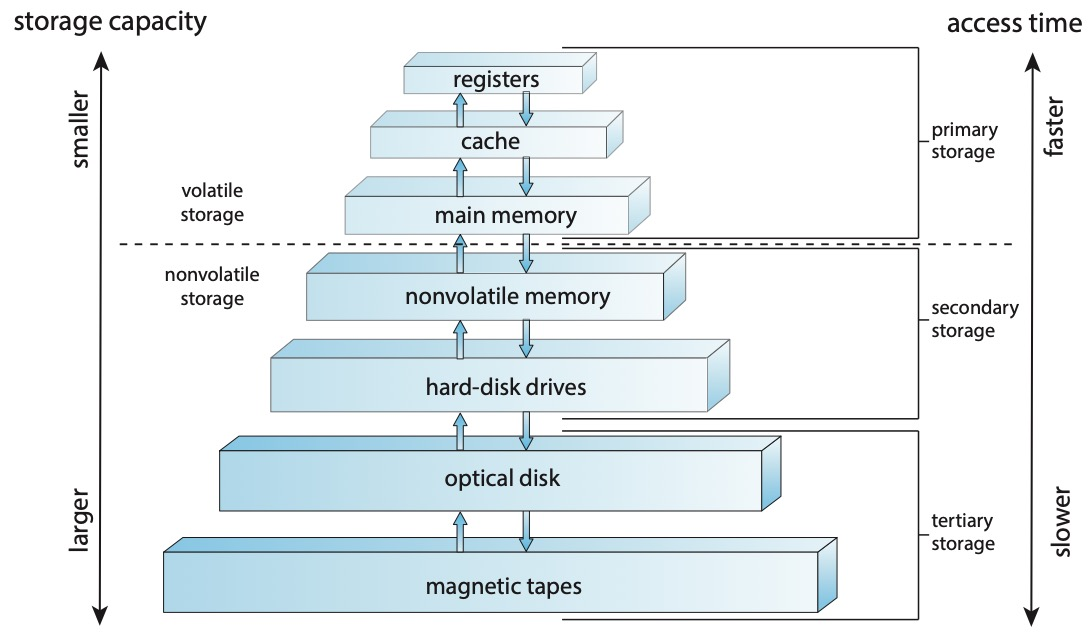
\includegraphics[width=0.48\linewidth]{assets/storage-hierarchy.jpg}
\end{figure}

\subsection{Cache}

La cache si inserisce tra il processore e la memoria principale, quando la CPU richiede un valore esso viene prima cercato nella cache:
\spacer
\begin{sitemize}
    \item \textbf{cache hit:} Il valore viene trovato e può essere restituito alla CPU rapidamente.
    \item \textbf{cache miss:} Il valore non viene trovato, quindi sarà necessario attendere la DRAM.

    Dopo aver recuperato il valore esso, e i valori adiacenti, vengono salvati nella cache, applicando una politica di rimpiazzo se la cache è piena.
\end{sitemize}

\spacer
L'obiettivo è quello di rendere il più grande possibile la percentuale di cache hit sul totale delle richieste.

Per ottenere questo è particolarmente importante sviluppare una \textbf{politica di rimpiazzo} efficace, due principi efficaci a questo scopo:

\spacer
\begin{sitemize}
    \item \textbf{Località spaziale:} È probabile che la CPU debba accedere alle celle adiacenti, come nel caso della lettura di un vettore. È quindi conveniente copiare non solo la cella, ma un intero blocco di memoria RAM.
    \item \textbf{Località temporale:} È più probabile che venga richiesto un dato che è stato chiesto poco prima.
\end{sitemize}

\subsubsection*{Livelli di Cache}
Spesso per ottimizzare i tradeoff della cache essa viene organizzata in livelli (L1, L2, ...) dove più basso è il livello più la cache è piccola e veloce.
Questo viene fatto perché una cache L1 è molto più costosa di una L2 e così via.


Normalmente possiamo dire che la cache di livello $i + 1$ contiene tutti i dati della cache di livello $i$

\begin{note}
    Le prestazioni della cache sono particolarmente importanti per prestazioni dell'intero sistema, se viene progettata in modo corretto può garantire che una percentuale dall'80\% al 99\% degli accessi si limiti ad essa, senza andare alla memoria RAM.
\end{note}

\subsubsection{Esempio}
Una microarchittetura con 3 livelli di cache può essere sturtturata nel seguente modo:

\spacer
\begin{sitemize}
    \item Una cache L1 interna alla CPU, che contiene una parte per le istruzioni, L1-I (16 Kbyte) e una parte per i dati L1-D (64 Kbyte).
    \item Una cache L2, esterna alla CPU, ma contenuta comunque nel package. Di dimensioni maggiori (512 Kb - 1 Mb)
    \item Una cache L3, presente sulla motherboard
\end{sitemize}

\spacer
Le cache L1 e L2, interne al package, hanno un bus riservato, aumentando così le prestazioni.

\begin{figure}[H]
    \centering
    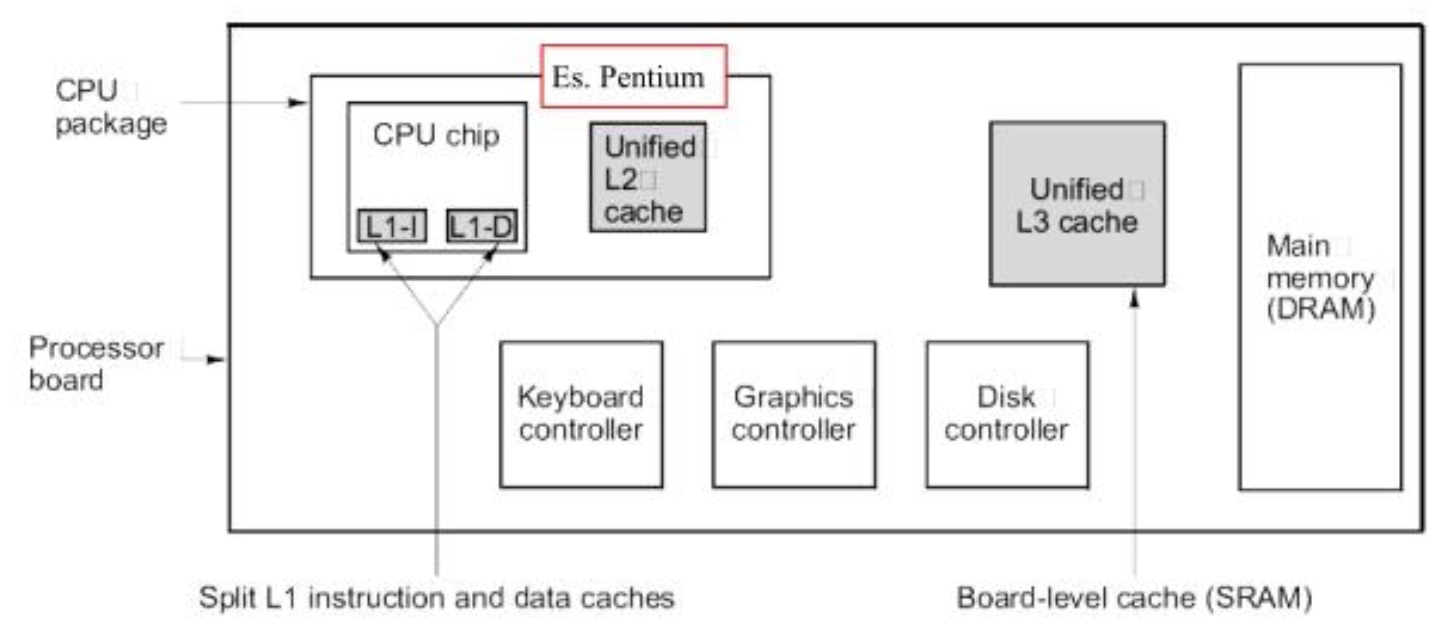
\includegraphics[width=0.5\linewidth]{assets/pentium-cache-architecture.jpeg}
\end{figure}


\section{Parallelismo}
A partire dal 1971 si è sempre rivelata vera la \textit{Legge di Moore} che afferma: "Il numero di transistor per chip, raddoppia ogni 18 mesi".

\spacer
Negli anni i progettisti di processori hanno affrontato con svariate tecniche il problema di tradurre l'aumento di densità dei transistor in un aumento delle prestazioni.

Ogniuna di queste tecniche ha pro e contro:
\spacer
\begin{sitemize}
    \item \textbf{Ridurre il numero di cicli}, quindi migliorare gli algoritmi. Questa è ancora una strada percorribile, ma in 60 anni di ricerca nell'ambito siamo riusciti a trovare soluzioni ottime per i problemi più rilevanti sull'ambito.
    \item \textbf{Aumentare la frequenza di clock} si rivela problematico per l'aumento di calore che viene prodotto, i processori moderni già producono la massima quantità di calore che può essere praticamente dissipata.
    \item Il \textbf{Parallelismo} è la strada che si è intrapresa negli ultimi anni, ha lo svantaggio di richiedere dell'overhead, quindi raddoppiare il numero di core non raddoppia le prestazioni, ma è la strada che permette di sfruttare l'aumento di densità nei transistor.

    Il parallelismo può avvenire al livello dell'istruzione, permettendo più operazioni all'interno dello stesso core (pipeline). Oppure può avvenire a livello di core, inserendo più core.
\end{sitemize}

\spacer
I metodi più utilizzati per realizzare il parallelismo sono:

\spacer
\begin{sitemize}
    \item \textbf{Componenti piccole} che \textbf{interagiscono fortemente tra loro}.

    Con questa soluzione viene parallelizzata la singola operazione (\textit{parallelismo fine-grained})

    Un esempio si trova nell'hyperthreading che permette ad una CPU di eseguire più processi allo stesso tempo.

    \item Un \textbf{piccolo numero di CPU grandi} dotate di \textbf{interconnessioni a bassa velocità}.

    Con questa tecnica l'elemento che viene parallelizzato è l'intero processo  (\textit{parallelismo course-grained})

    Ne sono esempi i sistemi multicore e la realizzazione di chip dedicati a specifiche operazioni.

\end{sitemize}

\begin{figure}[H]
    \centering
    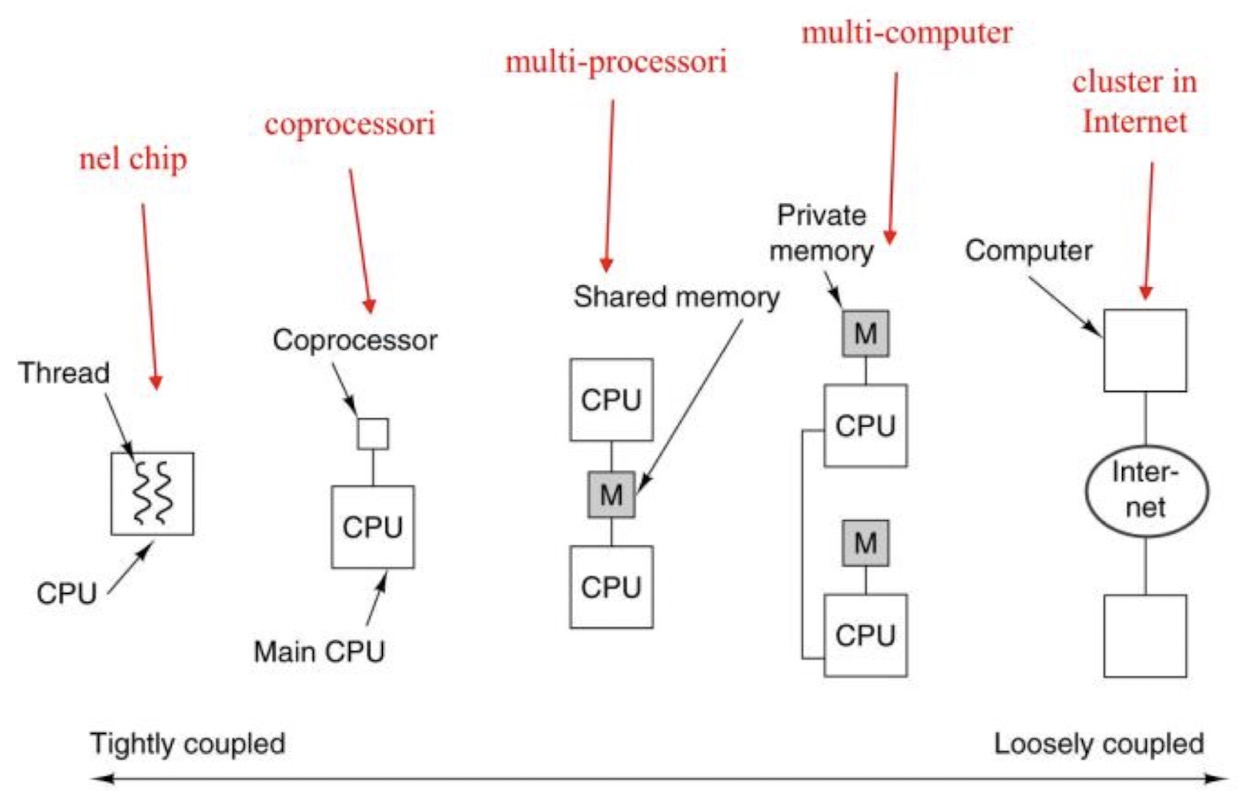
\includegraphics[width=0.45\linewidth]{assets/parallellismo.jpg}
\end{figure}

Gli elementi che caratterizzano il parallelismo, dal punto di vista hardware sono:
\begin{sitemize}
    \item \textbf{Natura e numero degli elementi di calcolo}, pochi elementi a prestazioni elevate, oppure molti elementi a basse prestazioni
    \item \textbf{Natura e numero degli elementi di memoria} La memoria viene divisa in moduli per permetterne l'accesso a tutti gli elementi di calcolo, il modo in cui viene divisa influenza il parallelismo
    \item \textbf{Modalità di connessione} Le connessioni possono essere di tipo statico, oppure dinamico, gestite tramite uno switch in grado di instradare i messaggi.
\end{sitemize}

\subsection{Implementazioni}
Il parallelismo può essere quindi implementato su più livelli:
\begin{sitemize}
    \item \textbf{A livello di istruzioni} tramite pipeline.
    \item \textbf{Multi-threading} Due thread vengono eseguiti contemporaneamente, una CPU virtualizza due CPU.
    \item \textbf{Multi-core} Consente il completo multi-threading di più processi.
    \item \textbf{Core Eterogenei} all'interno dello stesso chip, ognuno con funzionalità specializzate.
\end{sitemize}

\begin{note}
    Sia intel (a partire dall'architettura Ice Lake) che Apple (con i suoi Apple Silicon), implementano un'architettura ibrida, con core ad alte prestazioni e altri core per processi di minore importanza.
\end{note}
\section{Multiprocessori e MultiComputer}
Il modo forse più diretto per implementare il parallelismo è quello di aggiungere più processori, creando un \textbf{multiprocessore}.

Se essi condividono la stessa memoria essi possono essere trattati come un unico processore e sono un esempio di un sistema \textit{strongly coupled}.

\begin{figure}[H]
    \centering
    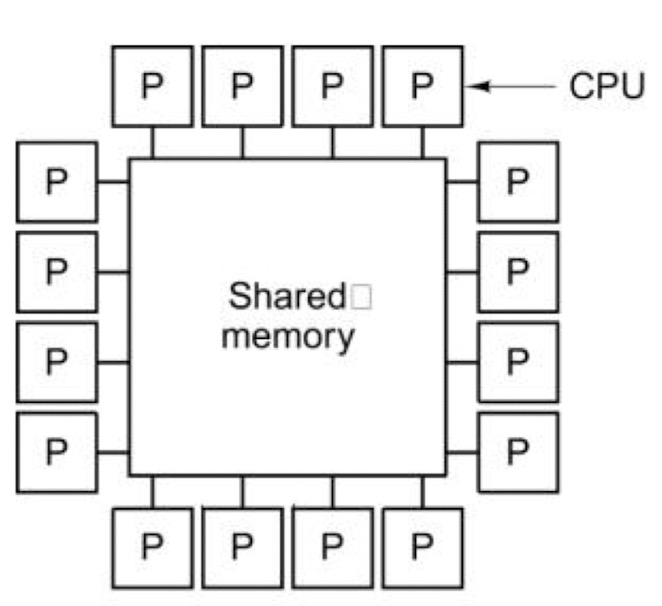
\includegraphics[width=0.28\linewidth]{assets/multiprocessore.jpg}
\end{figure}

Per inserire una potenza di calcolo ancora maggiore è necessario unire due o più multiprocessori in un \textbf{multicomputer}.

In questo caso risulta essere più complessa la programmazione, in quanto i sistemi sono \textit{loosely coupled} ed è necessario tenere conto degli overhead dello scambio di informazioni, ma a livello hardware sono molto più semplici da costruire a parità di core.

\begin{figure}[H]
    \centering
    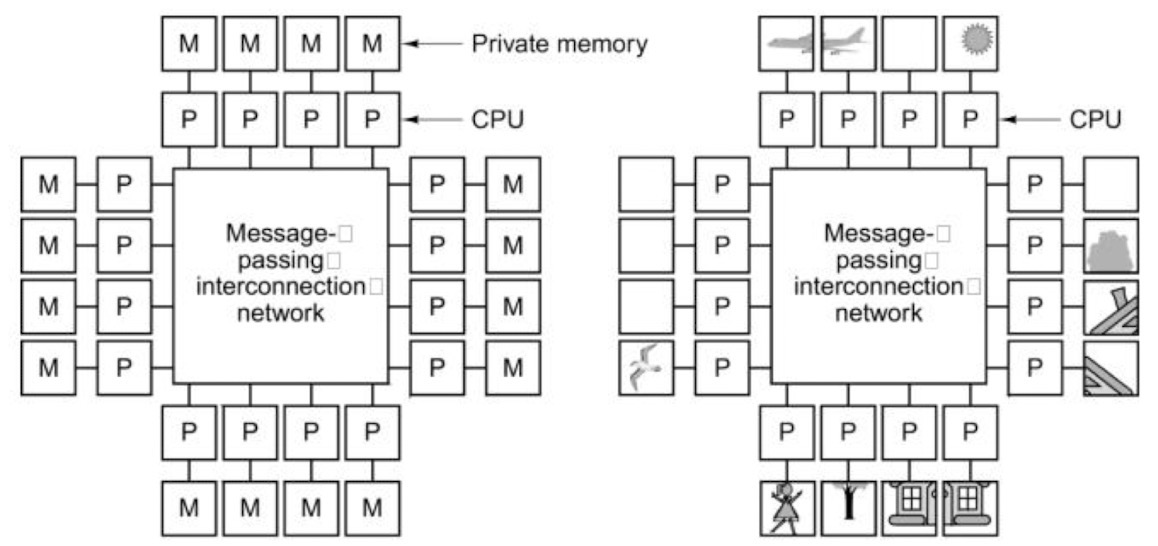
\includegraphics[width=0.62\linewidth]{assets/multicomputer.png}
\end{figure}

\begin{note}
    Quando due SoC sono connessi con una connessione con larghezza di banda sufficiente essi possono essere trattati come un unico chip. Ad esempio la serie Ultra dei chip Apple Silicon ha una connessione "DeepFusion" a 2.5 TB/s a bassa latenza.
\end{note}

\subsection{Topologia delle Connessioni}

In un sistema multicomputer la \textbf{topologia} delle connessioni tra i vari computer diventa di centrale importanza, si cercano le migliori prestazioni riducendo la quantità di connessioni necessarie.

\begin{figure}[H]
    \centering
    \begin{minipage}{0.45\textwidth}
        \subsubsection{Grado o fanout}
        Il numero di connessioni che passano per un nodo, un grado maggiore indica maggiori tolleranze a possibili interruzioni di rete.
    \end{minipage}
    \hfill
    \begin{minipage}{0.45\textwidth}
        \begin{figure}[H]
            \centering
            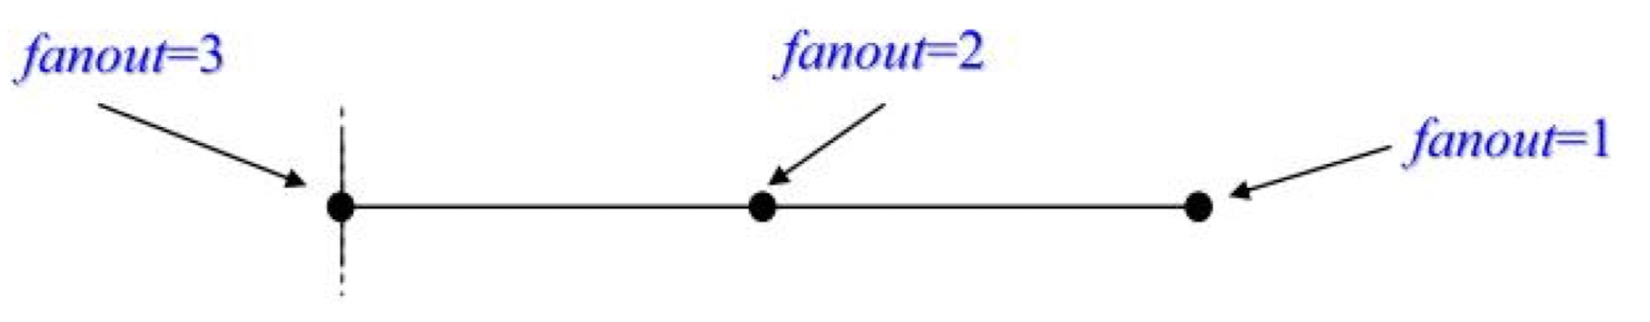
\includegraphics[width=1\linewidth]{assets/fanout.jpg}
        \end{figure}
    \end{minipage}
\end{figure}

\begin{figure}[H]
    \centering
    \begin{minipage}{0.45\textwidth}
        \subsubsection{Diametro}
        Il numero massimo di passaggi tra un nodo e un'altro in una rete, dà informazioni sul tempo di comunicazione nel caso peggiore.
    \end{minipage}
    \hfill
    \begin{minipage}{0.45\textwidth}
        \begin{figure}[H]
            \centering
            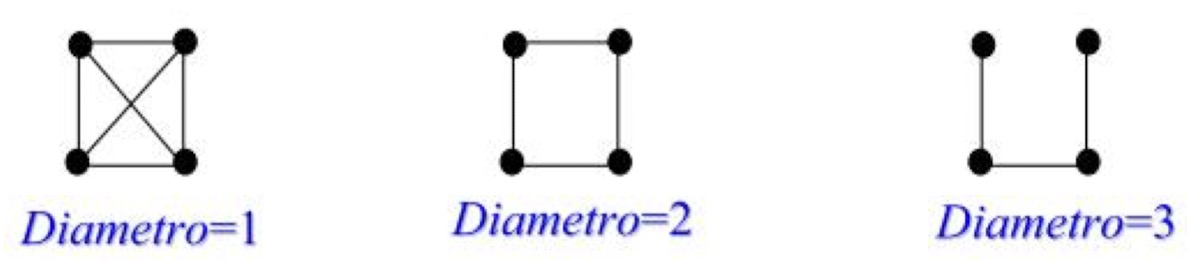
\includegraphics[width=1\linewidth]{assets/diametro.jpg}
        \end{figure}
    \end{minipage}
\end{figure}

\begin{figure}[H]
    \centering
    \begin{minipage}{0.45\textwidth}
        \subsubsection{Dimensionalità}
        Numero di assi che devono essere percorsi per arrivare dal un nodo ad un'altro (caso massimo).
    \end{minipage}
    \hfill
    \begin{minipage}{0.45\textwidth}
        \begin{figure}[H]
            \centering
            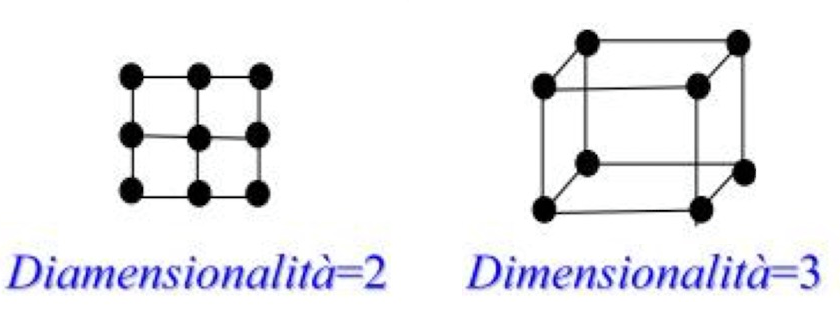
\includegraphics[width=0.65\linewidth]{assets/dimensionalita.png}
        \end{figure}
    \end{minipage}
\end{figure}

\begin{figure}[H]
    \centering
    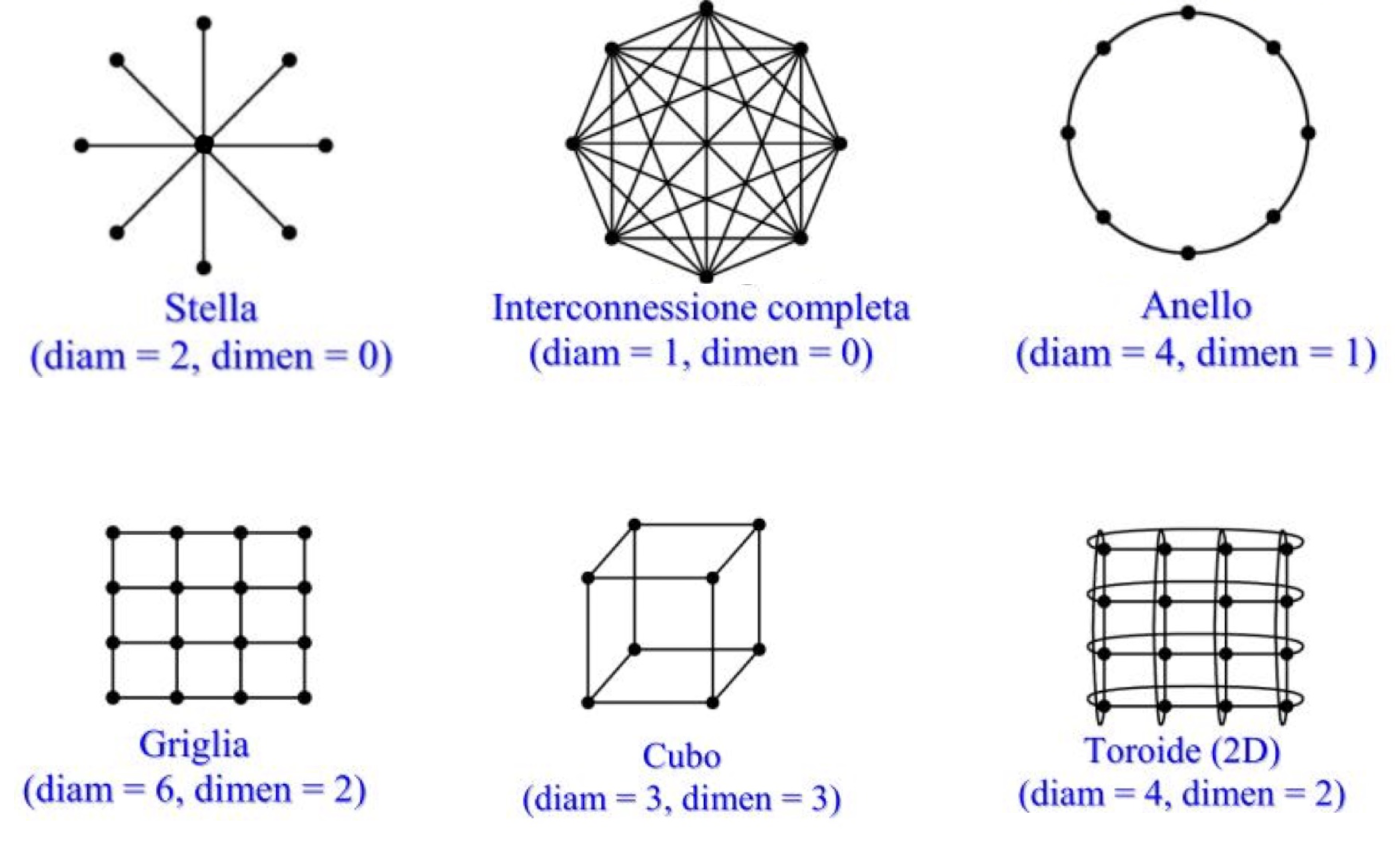
\includegraphics[width=0.5\linewidth]{assets/connessioni.png}
    \caption{Esempi di connessioni}
\end{figure}

\begin{note}
    Nei supercomputer nella maggior parte dei casi si opta per una connessione a toroide 3D, quindi ha dimensione 3, che porta un buon compromesso tra diametro e numero di connessioni.

    \begin{figure}[H]
        \centering
        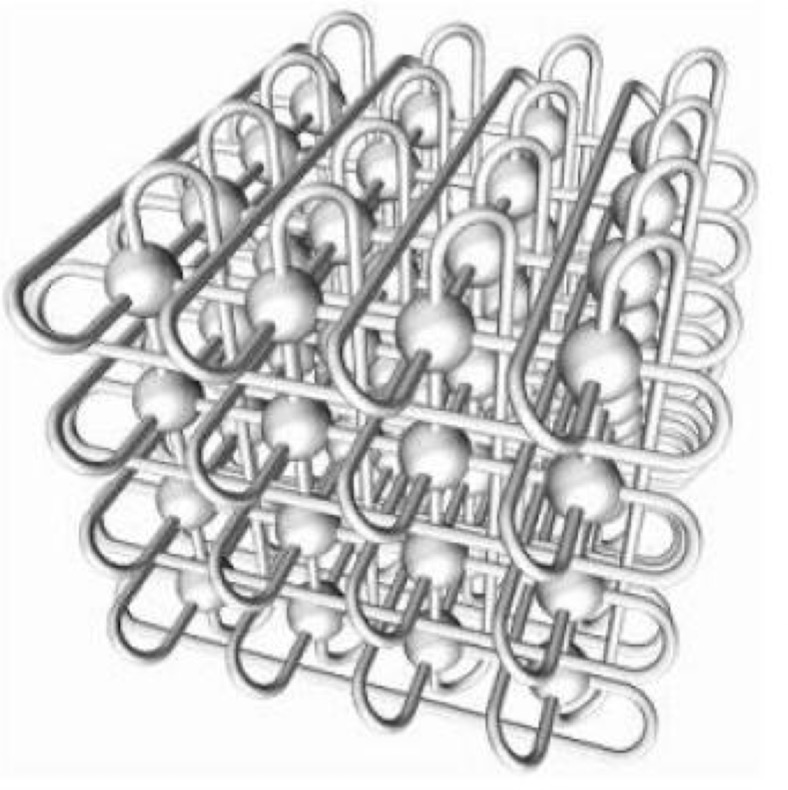
\includegraphics[width=0.3\linewidth]{assets/toroide3d.jpg}
        \caption{Toroide(3D)}
    \end{figure}
\end{note}

\subsection{Prestazioni}
Vogliamo calcolare quanto aumentano le prestazioni se applichiamo $n$ CPU allo stesso problema.

Ovviamente è impossibile ottenere un aumento delle prestazioni pari a $n$.

\spacer
\begin{sitemize}
    \item Esistono parti dei programmi \textbf{intrinsecamente sequenziali}.
    \item La \textbf{comunicazione}, per quanto efficiente, comporta dell'overhead.
    \item Gli \textbf{algoritmi paralleli} sono spesso sub-ottimi rispetto a quelli sequenziali.
\end{sitemize}

$$T_{es, parallelo} = f\cdot T_{es, sequenziale} + \frac{(1-f)\cdot T_{es, sequenziale}}{n}$$

dove $f$ è la frazione di codice sequenziale sul totale.

\subsubsection{Prestazioni e Connessioni}
Aumentare il numero di CPU spesso non è sufficiente per incrementare le prestazioni. È necessario avere un'architettura \textbf{scalabile}.

Delle buone struttura di topologia delle connessioni sono a griglia e a cubo, mentre quella ottimale è l'ipercubo, in quanto il diametro aumenta logaritmicamente rispetto al numero dei processori.

\subsection{Tassonomia o Classificazione dei sistemi}
Quella più utilizzata è quella ideata da Flynn nel 1972 che si basa sulla grandezza delle sequenze di numeri e di dati.

\begin{center}
    \begin{tabular}{ | c | m{2cm} | m{2cm} | c | }
        \hline
        Nome & \raggedright Sequenze di istruzioni & \raggedright Sequenze di dati & Esempi                         \\
        \hline \hline
        SISD & 1                                   & 1                             & Macchina di Von Neumann        \\
        SIMD & 1                                   & Molte                         & Computer Vettoriali            \\
        MISD & Molte                               & 1                             & Solo teoriche                  \\
        MIMD & Molte                               & Molte                         & Multiprocessori, Multicomputer \\
        \hline
    \end{tabular}
\end{center}

\subsection{Implementazioni}

\subsubsection{NUMA}
Spesso il fattore limitante al numero di processori che è possibile aggiungere ad un sistema è la dimensione del bus che porta alla memoria principale.

\spacer
Nell'architettura NUMA si fornisce ad ogni processore una \textbf{memoria locale} a cui può accedere con un suo bus separato.

Inoltre tutti i processori condividono gli stessi indirizzi fisici, quindi la comunicazione tra processori può avvenire facilmente tramite una connessione diretta.

\spacer

Questo rende molto più semplice scalare i sistemi e accelera i tempi di accesso tra il processore e la sua memoria, tuttavia l'accesso alla memoria di un'altro processore è molto rallentato.

\begin{figure}[H]
    \centering
    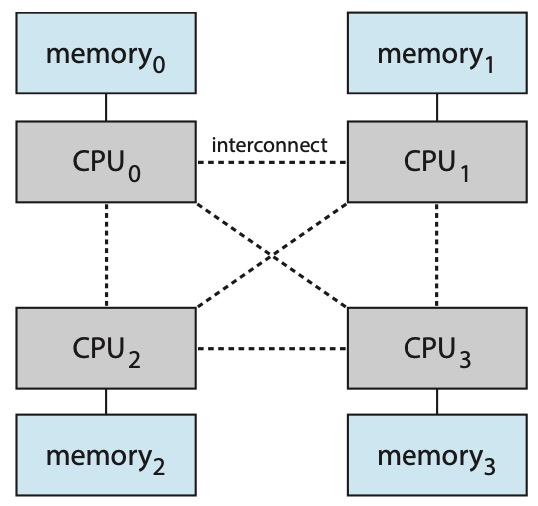
\includegraphics[width=0.3\linewidth]{assets/NUMA.jpg}
    \caption{Visualizzazione sistema NUMA}
\end{figure}

\subsubsection{Cluster}
In modo simile a quanto possiamo fare per più processori possiamo collegare due o più calcolatori completi. I quali possono condividere una memoria secondaria comune.
Questi sistemi sono debolmente accoppiati, quindi non tutte le operazioni possono sfruttare la completa potenza di calcolo.

Anche in questo caso è possibile creare cluster \textbf{asimmetrici} e \textbf{simmetrici}, i primi possiedono un nodo che ha l'unica funzione di gestire gli altri rimanendo in uno stato di attesa attiva, mentre nei secondi tutti i nodi eseguono le applicazioni e si controllano reciprocamente.

\begin{figure}[H]
    \centering
    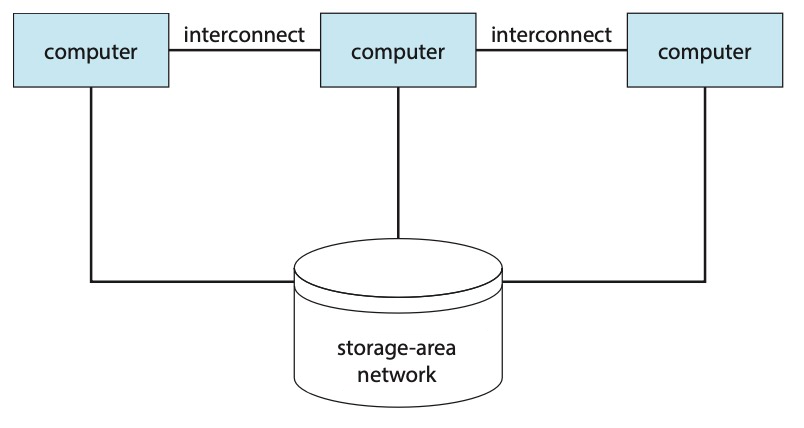
\includegraphics[width=0.5\linewidth]{assets/cluster.png}
    \caption{Cluster}
\end{figure}

\begin{note}
    Questo risulta essere particolarmente utile nel caso di sistemi che devono essere sempre operativi, anche nel caso di un malfunzionamento di uno dei computer il servizio non viene interrotto.

    \spacer
    I Cluster vengono utilizzati anche nell'\textit{High performance computing}, ma le applicazioni devono essere scritte appositamente per poter sfruttare tutte le prestazioni messe a disposizione dal cluster.
\end{note}

\subsection{Coprocessori}
Un coprocessore è un processore \textbf{indipendente} che esegue compiti specializzati sotto il controllo del processore principale.

\spacer
\begin{sitemize}
    \item \textbf{Coprocessori di rete:} Specializzati per gestire ad alta velocità i pacchetti di rete.
    \item \textbf{Crittoprocessori:} Consentono di cifrare/decifrare velocemente flussi di dati.
    \item \textbf{Graphical Processing Unit (GPU):} Consente di processare una gran quantità di dati video e grafica 3D. Una singola GPU può contenere fino a qualche migliaio di core grafici.
    \spacer
    Le GP-GPU, \textit{general purpose GPU} grazie a linguaggi di programmazione quali CUDA e OpenCL possono essere facilmente utilizzate per operazioni floating point, rendendole così di grande importanza nell'high performance computing.
    \spacer
    Per ottenere questo tipo di schede grafiche è stato necessario convertire i core per renderli compatibili alle specifiche IEEE per l'aritmetica a singola e doppia precisione. Inoltre è stato necessario fornire accesso in lettura e scrittura alla memoria principale.
    \item \textbf{Tensor Processing Unit (TPU):} Un coprocessore dedicato alle reti neurali per il \textit{deep learning}.
    \item \textbf{Field Programmable Gate Array (FPGA):} È un dispositivo che permette di implementare algoritmi in hardware, tramite software.

    Presenta una serie di blocchi logici configurabili e sono ideali per lo sviluppo e per dei prototipi rapidi.
\end{sitemize}

\section{High Performance Computing}
Con \textit{High Performance Computing} (\textit{HPC}) si intende l'utilizzo di multiprocessori o cluster per effettuare computazioni concorrenti tale che porti a throughput ed efficienza elevati.

Hardware e Software devono essere strettamente collegati per permettere l'utilizzo massivo della parallelizzazione

\subsection{Parallelismo}
Esistono due tipi principali di parallelismo:
\begin{sitemize}
    \item \textbf{Parallelismo delle task} Quando diverse task possono essere esguiti indipendentemente, in questo caso possonoe essere facilmente allocate su diversi core.
    \item \textbf{Parallelismo dei dati} Quando si può operare indipendentemente su porzioni distinte dei dati, in modo da poter suddividere le porzioni su più core.
\end{sitemize}

\subsection{Utilizzo delle GPU}
Mentre per le CPU l'incapacità di aumentare la frequenza e lo spostamento verso sistemi sempre più parallelizzati ha portato ad una riduzione del miglioramento delle performance, le \textbf{GPU}, nate con l'obiettivo di \textbf{elaborare processi parallelamente} hanno continuato a seguire quanto ipotizzato da Moore.

\spacer
Grazie all'architettura \textit{CUDA} le schede video NVIDIA hanno reso possibile la semplice scrittura di programmi altamente paralleli.

Ad oggi si utilizzano CPU solo quando non si può ottenere una grande parallelizzazione, mentre GPU quando è possibile distribuire il carico su un enorme numero di core relativamente poco potenti.

\spacer
Alcune computazioni possono benificiare da un approccio misto tra CPU e GPU, in questo caso il trasferimento dei dati da una memoria all'altra può causare dei rallentamenti anche importanti.

Per questo è in alcuni casi conveniente utilizzare una \textbf{memoria condivisa} così da eliminare questo overhead.

Un'implementazione della memoria condivisa si vede nei chip Apple Silicon che presentano un'unica pool di memoria da cui CPU e GPU attingono.

\begin{figure}[H]
    \centering
    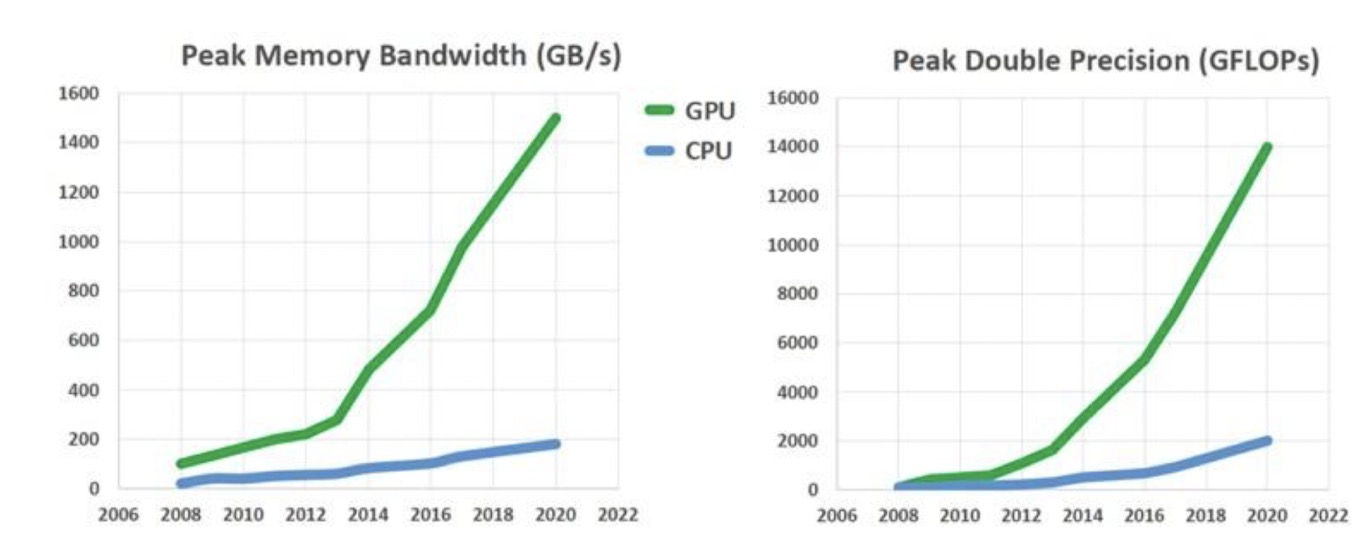
\includegraphics[width=0.65\linewidth]{assets/gflops-gpu-cpu.jpg}
    \caption{Gflops di CPUs e GPUs nel tempo}
\end{figure}

\subsection{TPU}
Da qualche anno Google si è dedicata allo sviluppo di una nuova tipologia di chip chiamati \textit{Tensor Processing Unit}, i quali hanno un set di operazioni ancora più ridotto rispetto alle GPU, ogni core ha quindi una superficie minore, rendendo così possibile stiparne un numero maggiore sullo stesso chip.

\spacer
Questi processori sono indirizzati al \textbf{Machine Learning}, in particolare all'esecuzione di algoritmi per l'allenamento di reti neurali

\subsection{FPGA}

I \textit{Field Programmable Gate Array} sono dei dispositivi che contengono dei blocchi logici configurabili, essi consentono di programmare dell'hardware per fornirgli particolari funzionalità.

\spacer
Essi permettono di implementare funzioni in hardware, con tutti i benfici che questo porta, senza dover sostenere i costi di fabbricazione di un chip.


